\chapter{Dokumentacja}

\section{Diagramy klas}

\begin{center}
	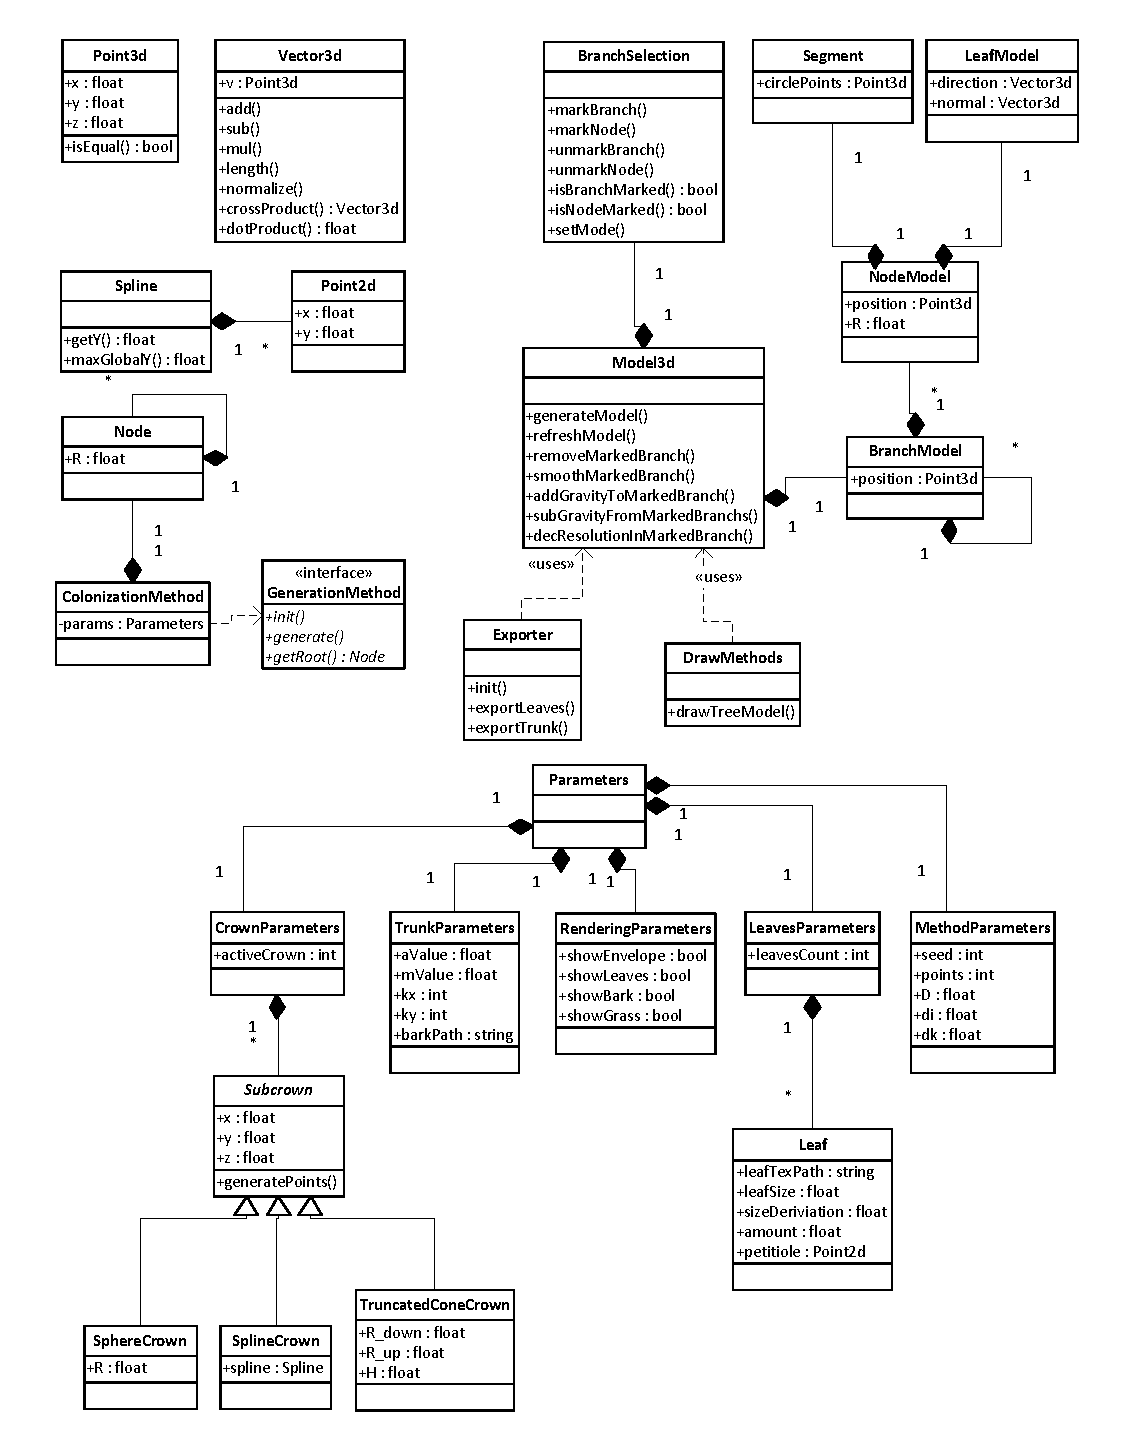
\includegraphics[scale=0.55]{images/treemaker_uml}
	\label{treemaker_uml}
\end{center}

\section{Eksport modelu}
Ponieważ format danych używany w programie nie jest zgodny z powszechnie uznanymi formatami modeli trójwymiarowych, aby zachować kompatybilność należy przeprowadzić eksport modelu do 
formatu zewnętrznego. Format .OBJ zgodnie wymaganiami jest obsługiwany przez program Blender.
Został on opracowany przez firmę Wavefront Technologies i ze względu na swoją prostotę stał się szybko
popularny wśród programów do obróbki grafiki trójwymiarowej. Na format składa się tekstowy z rozszerzeniem .obj 
zawierający opis geometrii obiektu, dodatkowo format przewiduje odwołanie do pliku z rozszerzeniem .mtl zawierającym
opis materiałów (kolorów i tekstur).


\subsection{Struktura pliku .obj}
Plik jest podzielony na linie, z czego każda linia moze zawierać:
\begin{itemize}
\item '\#' : komentarz 
\item mtllib [nazwa pliku .mtl] :odwołanie do pliku z materiałami
\item usemtl [nazwa materiału]  :nakaz uzycia materiału
\item o [nazwa obiektu]         :definicję obiektu
\item g [nazwa grupy]           :definicję grupy: 
\item v [x] [y] [z]             :współrzędne wierzchołka
\item vn [x] [y] [z]            :współrzędne wektora normalnego
\item vt [x] [y]                :współrzędne tekstury
\item f [v1/vn1/vt1] [v2/vn2/vt2] [v3/vn3/vt3] :definicja trójkąta 
\end{itemize}
Warto nadmienić, iż przy definiowaniu trójkątów podajemy indeksy (numerowane od 1) poszczególnych współrzędnych w znajdujących się w pliku.
Istotne jest również to, iż współrzędne tekstury i wektora normalnego trójkąta są opcjonalne, a sam wektor normalny może być odtworzony poprawnie,
nawet jeśli nie został zawarty w pliku dzięki podaniu współrzędnych wierzchołków zgodnie z ruchem wskazówek zegara.


\subsection{Struktura pliku .mtl}
Plik .mtl może zawierać definicje wielu materiałów. Podobnie jak plik .obj jest to plik tekstowy z informacjami znajdującymi
się w kolejnych liniach mogących zawierać:
\begin{itemize}
\item '\#' : komentarz 
\item newmtl [nazwa materiału]: definicja materiału
\item Ka [r] [g] [b]: ambient kolor
\item Kd [r] [g] [b]: diffuse kolor
\item Ks [r] [g] [b]: specular kolorów
\item Ns [x]        : specular cooef
\item d  [x]        : przezroczystosc
\item map\_Ka [nazwa pliku]: tekstura 
\end{itemize}


\subsection{Procedura eksportu}
Model drzewa jest eksportowany w dwóch etapach, jako dwie osobne grupy jednego obiektu. Pierwszą grupę stanowi pień drzewa, drugą natomiast jego liście.
Pozwala to na użycie różnych tekstur dla tych elementów drzewa. Program grupuje współrzędne wierzchołków i tekstur by zmniejszyć rozmiar tworzonego pliku, a następnie
zapisuje je do pliku \{models/tree0.obj\}. Dodatkowo program tworzy plik \{models/tree0.mtl\} zawierający opis materiałów i ścieżki do tekstur. 
\section{Opis interfejsu użytkownika}

\subsection{Okno główne}
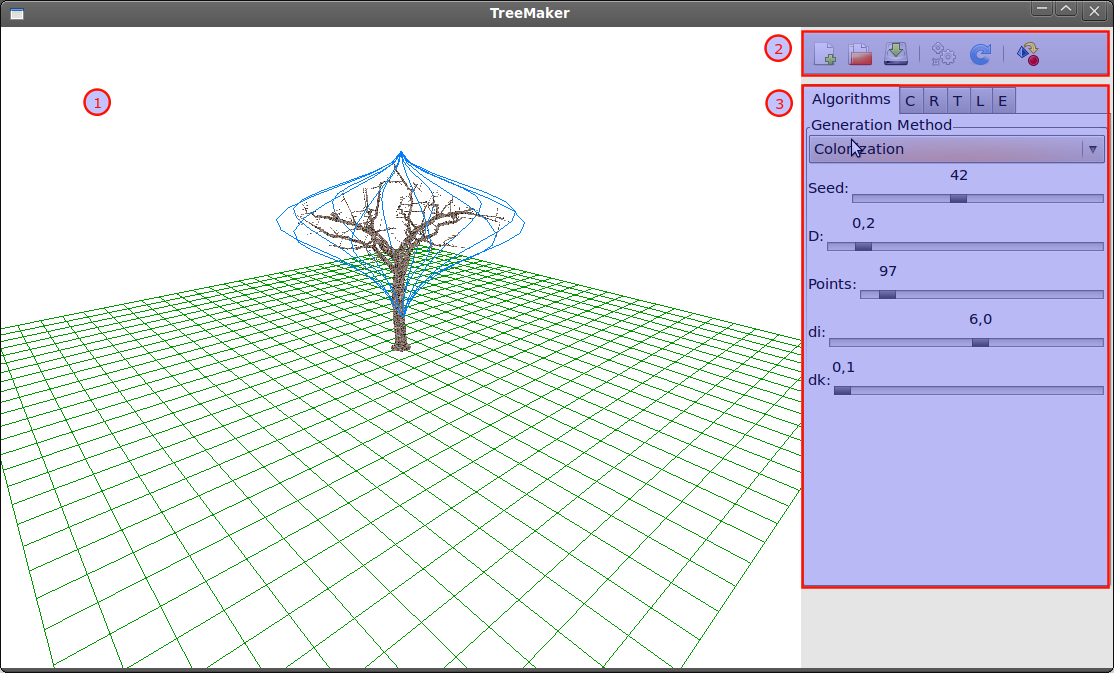
\includegraphics[width=120mm]{images/gui/main_window.png}
\begin{enumerate}
	\item {Podgląd wygenerowanego drzewa.}
	\item {Toolbar.}
	\item {Panel z ustawieniami generatora.}
\end{enumerate}

\subsection{Podgląd wygenerowanego modelu}
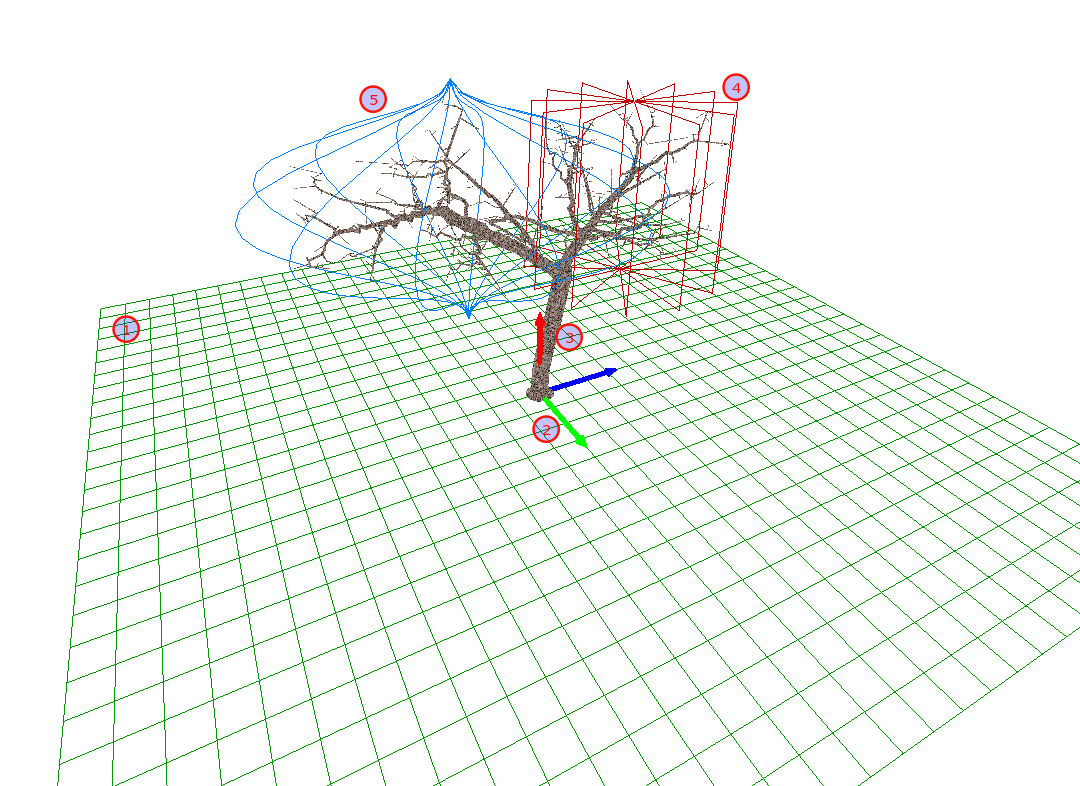
\includegraphics[width=120mm]{images/gui/model_view.png}
\begin{enumerate}
	\item {Siatka wyznaczająca poziom ziemi.}
	\item {Układ współrzędnych.}
	\item {Model drzewa.}
	\item {Aktywna korona.}
	\item {Nieaktywna korona.}
\end{enumerate}

\subsection{Toolbar}
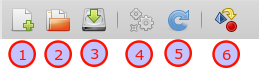
\includegraphics[width=50mm]{images/gui/toolbar.png}
\begin{enumerate}
	\item {Resetuj konfigurację.}
	\item {Wczytaj konfigurację.}
	\item {Zapisz konfigurację.}
	\item {Generuj nowy model.}
	\item {Odśwież model.}
	\item {Eksportuj model.}
\end{enumerate}

\subsection{Opcje algorytmu}
\begin{tabular}{lr}
\parbox[b]{95mm}{
\begin{enumerate}
	\item {Wybór algorytmu generującego drzewo.}
	\item {Ziarno generatora pseudo-losowego.}
	\item {Odległość pomiędzy sąsiednimi węzłami w drzewie.}
	\item {Liczba atraktorów, z których generowane jest drzewo.}
	\item {Influence distance - promień przyciągania atraktorów do drzewa.}
	\item {Kill distance - ?.}
\end{enumerate}
} &
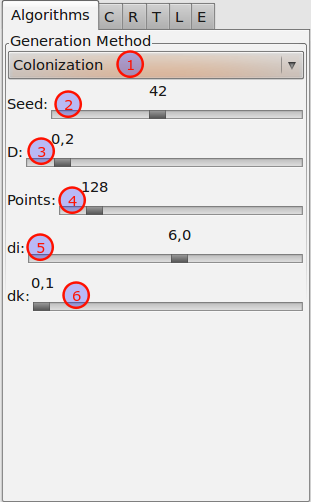
\includegraphics[width=35mm]{images/gui/algorithms_panel.png} \\
\end{tabular}



\subsection{Opcje korony}
\begin{tabular}{lr}
\parbox[b]{95mm}{
\begin{enumerate}
	\item {Typ korony (sfera, ścięty stożek, bryła obrotowa oparta o krzywą sklejalną trzeciego stopnia).}
	\item {Dodaj koronę.}
	\item {Lista dodanych koron.}
	\item {Współrzędna X wybranej korony.}
	\item {Współrzędna Y wybranej korony.}
	\item {Współrzędna Z wybranej korony.}
	\item {TODO widok dla każdego typu korony}
\end{enumerate}
} &
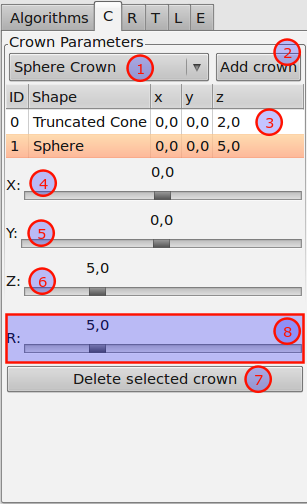
\includegraphics[width=35mm]{images/gui/crown_panel.png} \\
\end{tabular}


\subsection{Opcje wyświetlania}
\begin{tabular}{lr}
\parbox[b]{95mm}{
\begin{enumerate}
	\item {Wyświetla dodane korony.}
	\item {Wyświetla liście.}
	\item {Wyświetla korę.}
	\item {Wyświetla trawę.}
\end{enumerate}
} &
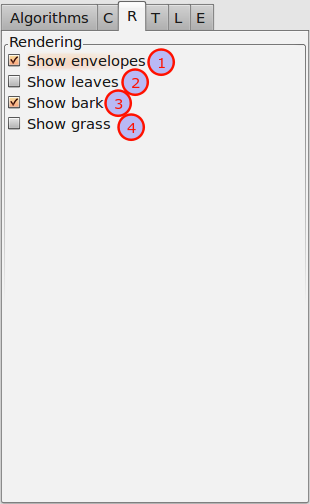
\includegraphics[width=35mm]{images/gui/rendering_panel.png}\\
\end{tabular}

\subsection{Opcje pnia}
\begin{tabular}{lr}
\parbox[b]{95mm}{
\begin{enumerate}
	\item {Współczynnik $radius factor$. Wpływa na grubość pnia przy łączeniu gałęzi.}
	\item {Współczynnik $a$.}
	\item {Współczynnik $m$.}
	\item {Liczba punktów tworzących segment.}
	\item {Liczba tekstur potrzebną do owinięcia pnia.}
	\item {Stosunek rozmiaru tekstury do odległości mierzonej wzdłuż pnia.}
\end{enumerate}
} &
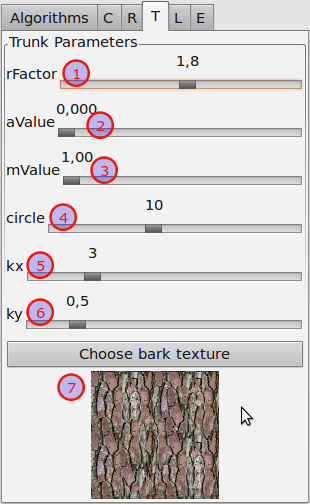
\includegraphics[width=35mm]{images/gui/trunk_panel.png}\\
\end{tabular}

\subsection{Opcje liści}
\begin{tabular}{lr}
\parbox[b]{95mm}{
\begin{enumerate}
	\item {Liczba liści doczepianych do wygenerowanego modelu.}
	\item {Lista rodzajów liści.}
	\item {Rozmiar danego liścia.}
	\item {?}
	\item {Współczynnik wpływający na liczbę liści danego typu.}
	\item {Dodawanie nowego typu liścia.}
\end{enumerate}
} &
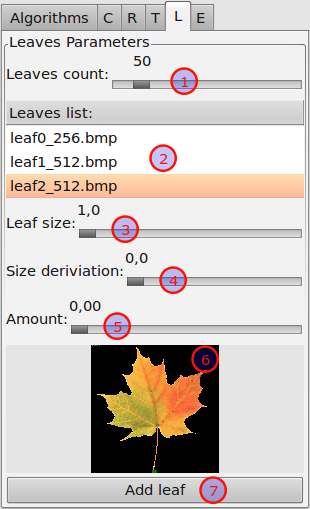
\includegraphics[width=35mm]{images/gui/leaves_panel.png}\\
\end{tabular}




\subsection{Edytor}
\begin{tabular}{lr}
\parbox[b]{95mm}{
\begin{enumerate}
	\item {Tryb zaznaczania gałęzi - odpowiednio: cała gałęź, od punktu do końca gałęzi oraz od punktu do punktu}
	\item {Zastosuj dla wszystkich dzieci - edycji podlegają też gałęzie wychodzące z edytowanego fragmentu}
	\item {Przycinanie gałęzi}
	\item {Wygładzanie gałęzi (zwiększana jest rozdzielczość gałęzi)}
	\item {Zmniejszanie gałęzi}
	\item {Dociążanie gałęzi}
	\item {Działanie przeciwne do opcji 6}
\end{enumerate}
} &
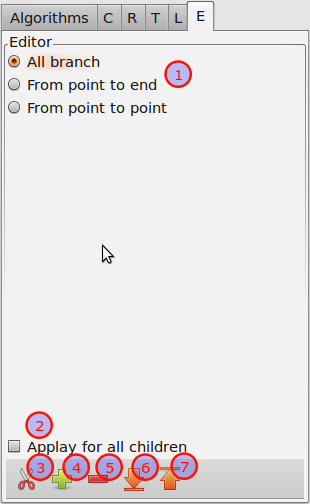
\includegraphics[width=35mm]{images/gui/editor_panel.png} \\
\end{tabular}

\section{Kompilacja projektu}
\subsection{Wymagane biblioteki}
Zgodnie z wymaganiami programi powinien posiadać możliwie małą ilość zależności. System powinien posiadać kompilator GCC oraz bibliotekę GTK+ z rozszerzeniem do obsługi OpenGL.
Poniżej przedstawiono dokładne wersje bibliotek wymagane przez program.
\begin{itemize}
\item GTK+ 2.2
\item GTKGLEXT 1.2
\item MESA 7.8
\item GCC 4.4.4
\end{itemize}
\subsection{Uruchomienie}
Źródła programu zostały załączone na płycie CD, ponadto znajdują się na stronie https://code.google.com/p/treemaker/source/browse/.\\
Po ich pobraniu wystarczy wydać polecenie make w katalogu ze źródłami by rozpocząć kompilację programu. Jeśli przebiegła ona pomyślnie został utworzony
program wykonywalny o nazwie treemaker.
